\chapter{Accessibility \who{Ziemke}}
\label{ch:accessibility}
% ##################################################################################################################

\hfill \textbf{Author:} Dominik Ziemke

\begin{center} 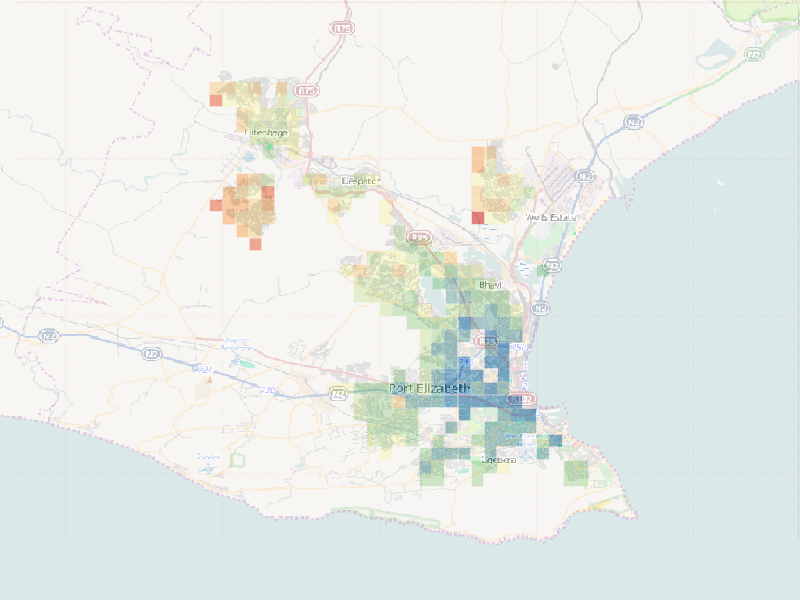
\includegraphics[width=1.\textwidth, angle=0]{extending/figures/accessibility/w_freeSpeed_snapshot.png} \end{center}

\createStandardInformation{accessibility}{\kai{todo}}{accessibility}{\kai{todo}}

% ##################################################################################################################
The term accessibility is widely used in the context of transport and infrastructure planning. The improvement of accessibility is often stated as a central goal of proposed transport or infrastructure schemes. In contrast to the ubiquitous use of the term accessibility, however, approaches to the quantitative analysis of accessibility are comparatively rare. This is striking since first such approaches appear to have been undertaken at the latest in the 1950s (cite Hansen ????????????). Likewise, it is notable that the development of gravity models, which have since then been the most prominent and widely-applied type of destination choice models, has originally been intertwined with quantitative approaches to accessibility analysis.

Today, methods to assess the quality of accessibility (cite BBSR, TUHH, TUM, Curtis, ... ??????????) are mainly used in superordinate planning procedures like regional planning, where a central goal is to provide citizens with a certain quality of access to various services. Curtis et al. (cite Curtis... ??????) also argue that accessibility-based analysis methods may be suitable to overcome the deficits that traditional transport analysis methods possess in terms of analyzing transport policies that are not construction-based, e.g. transport demand management schemes.

\mnote{typology}
Depending on the concrete definition of quantitative accessibility measures, the explanatory power of the result varies widely.
%
As pointed out by \citet{NicolaiNagel2012HiResAccessibilityMethodInBook} (\citep[see also][]{GeursRitsema2001AccessibilityMeasures,Geurs2004AccessibilityReview}), quantitative indicators can rely on the following approaches:
%
\begin{enumerate}
\item An \textbf{activity-based} or \textbf{land-use-based} approach focuses on
the distribution of possible activity locations (land use). One can, for instance,
base calculations on the number and spatial distribution of activity opportunities
like shopping locations or workplaces within a certain distance.
%
\item An \textbf{in\-fra\-struc\-ture-based} or \textbf{transport-based} approach takes into account the effort to travel from a given origin to a given destination and 
can be based on performance characteristics of the transport system, e.g. the
average speed by mode at certain locations. If one considers, for instance, the
number of shopping locations or workplaces under a defined travel time threshold,
the activity-based and the infrastructure-based approaches can be combined.
%
\item A \textbf{temporal} component, which considers the availability of activities at different times-of-day, may be added.
%
\item An \textbf{individual} approach to accessibility computations can be
obtained by addressing different needs and opportunities of different socio-economic groups, e.g. different income groups.
%
\item A \textbf{utility-based} measurement of accessibility reflects the
(economic) benefits, as the maximum expected utility, that someone gains
from access to spatially distributed opportunities
\citep{GeursRitsema2001AccessibilityMeasures,deJongEtAl2007LogsumTRA}. The
typical example is the logsum term, which is discussed in ??????.
\end{enumerate}
%
%%%%%%%%%%%%%%%%%%%%%%%%%%%%%%%%%%%%%%%%%%%%%%%%%%%%%%%%%%%%%%
%
\mnote{Portfolio of opportunities}
Established and frequently applied approaches to accessibility analyses often calculate travel times to the next facility that offers a particular type of service (e.g. travel time to the next airport or next hospital, e.g. BBSR ????????) and define this travel time as the accessibility (OR use this as a proxy for accessibility....????).

While giving useful insights into the supply of the population with certain services, one can argue, however, that such approaches do not reflect the set of options, which a citizen can select from, very well. The measure will
arguably become more insightful, if not only the impedance to reach \textit{the nearest} facility serving a particular need is taken into account, but if instead a set of multiple reachable facilities serving the same need is considered. This is due to the fact, that different facilities of the same type may offer a  service in different qualities. Also, services may become more beneficent when combined with complementary services provided by another facility of the same type. For instance, a person wishing to make a holiday trip by airplane will likely take into account several airports in her/his vicinity when planning a journey instead of just looking at the flights offered from the nearest airport. Therefore, the accessibility to airports should be made dependent on the impedances to reach all of these airports instead of just the impedance to reach the nearest one. Facilities offering medical services may serve as another example. Only taking into account the nearest hospital may already be sufficient when looking at unsophisticated services like first aid, which can be assumed to be available at almost \textit{any} hospital. In most other cases, however, the the supply with medical services will be better represented by considering several hospitals in the vicinity because they are likely to offer different kinds of medical treatment that complement each other. Therefore, all reachable hospitals should be considered when calculating accessibilities of medical facilities instead of just taking into account the closest hospital.

In order to account for the multitude of facilities serving a given need, a (weighted) sum over the accessibilities of several facilities of a given type appears reasonable. The (quantitative) accessibility measure in the MATSim accessibility extension is of the mathematical form
\begin{equation}
A_i = g\Big( \sum_j a_j \, f(c_{ij}) \Big) \ ,
\label{eq:accessibility:basic}
\end{equation}
where the sum goes over all possible destinations (opportunities) $j$, $a_j$ is an indicator of the attractiveness of the opportunity, $c_{ij}$ is the generalized cost of travel to get from $i$ to $j$, $f(c)$ is an impedance function that typically decreases with increasing distance, and $g(.)$ is an arbitrary, but typically monotonically increasing, function.  That is, the accessibility at $i$ is computed from a weighted sum over all possible destinations, where the weight is the product of the destination's attractiveness and the ease to get there.

\mnote{ingoing vs. outgoing accessibility}
It is important to note that the above-defined measure quantifies how good the accessibility to certain services \textit{from} a given location $i$ is. This kind of accessibility could be referred to as "outgoing" accessibility, while a measure of "ingoing" accessibility would quantify how well a given location $i$ is accessible from other locations. Nicolai and Nagel \citet{NicolaiNagel2012HiResAccessibilityMethodInBook} discuss under which circumstances both measures are the same.

\mnote{uncongested vs. congested network}
As mentioned above, accessibility computations are oftentimes based on travel times, which serve as an impedance measure (cite BBSR ????????????). The calculation of the travel time can, however, vary. The most simple approach to calculate a travel time between two locations is measuring the Euclidian distance (beeline distance) between these two locations are by the means of some average speed approximate the travel time between these two locations. This has obvious disadvantages as, for instance, the quality of the transport infrastructure or topographic obstacles are not considered.

These disadvantages can be overcome by calculating actual travel routes and corresponding travel times on a network that represents the real-world transport infrastructure. While this calculation is obviously already possible by only considering transport supply, i.e. the transport network (e.g. BBSR ?????), its expressiveness can be further increased by additionally taking into account transport demand as well. This is useful because travel times increase with raising levels of demand on the network, which, in turn, cause reduced accessibilities as travelers need higher amounts of time to reach a given location. To operationalize this, a transport simulation which represents the interaction of transport supply and demand is needed. This is one major argument for the integration of an accessibility extension into the MATSim framework.

This way, the accessibility computation can be made dependent upon time-of-day, which is useful in contexts were levels of transport demand varies significantly over the course of the day, for instance when pronounced morning and afternoon peaks exist. Likewise, accessibility changes related to transport policies and corresponding reaction of decision makers may be considered.

\mnote{spatial resolution, zones vs. points}
In contrast to many other transport simulations, MATSim is not zone-based, but based on coordinates (see section ?????). Therefore, the accessibility computation within MATSim can also be conducted independent of any zonation system and, instead, be based on points or a raster with arbitrary granularity. This avoids several issues that may arise if accessibility computations are based on zones (see \citep[e.g.][]{NicolaiNagel2012HiResAccessibilityMethodInBook}) as it is done by the majority of other quantitative accessibility computations \citep[e.g.][]{Curtis, BBSR, LiuZhu2004AccessibilityAnalyst} (?????). Being raster- or coordinate-based, the outcome of the MATSim accessibility computation can be considered as an accessibility field,
i.e.\ as a measure continuously varying in space, $A(x,y)$, where $x$ and $y$
are the coordinates.  As is common in many areas of science, such
fields can be visualized by calculating the values on regular grid
points, and then using an averaging plotting routine. An example of such a visualization is shown in figure ????.

\mnote{econometric interpretation}
As pointed out by Curtis (????????????????) accessibilities can serve as an evaluation measure for transport policies. While most measures today rely on characteristics of the infrastructure, accessibility indicators are a holistic measure, which explicitly observes the interrelationship between transport and land use.

To make this measure most expressive in terms of econometric evaluation (e.g. cost-benefit analyses), it seems sensible to adapt equation \ref{eq:accessibility:basic} as follows: $g(.) = \ln(.)$, $a_j = 1$, $f(c_{ij}) = e^{-c_{ij}}$, and $-c_{ij} = V_{ij}$. Thus, equation \ref{eq:accessibility:basic} becomes
\begin{equation}
A_i := \ln \sum_k e^{V_{ik}} \ ,
\label{eq:accessibility:logsum0}
\end{equation}
where $k$ goes over all possible destinations, and $V_{ik}$ is the
disutility of travel in order to get from location $i$ to location
$k$. Equation \ref{eq:accessibility:logsum0} is the so-called logsum term and has an econometric interpretation as the expected maximum utility \citep[e.g.][]{Ben-AkivaBook}. It can be derived as follows: Assume that the full utility of location $k$, seen from $i$, is $U_{ik} = V_{base} + V_{ik} + \epsilon_{ik}$, where $V_{base}$ is a constant base utility for doing the activity at any location, $V_{ik}$ is the systematic ($=$ observed) disutility to travel to location $k$, and $\epsilon_{ik}$ is a random term which picks up the randomness of the travel disutility and, more importantly, also the utility fluctuations around $V_{base}$.  Under the typical assumption that the $\epsilon_{ik}$ are independent and identically Gumbel-distributed random variables, the expectation value of $U_{ik}$ becomes
\begin{equation}
E(U_i) = E(\max_k U_{ik}) = \ln \sum_k e^{V_{ik}} + Const \equiv A_i + Const \ .
\end{equation}
$Const$ is an integration constant, which can be dropped as it is the same for all locations. $A_i$ may also be negative.




\mnote{data}
free data

\mnote{applicability, useability}

\mnote{more}


%Aufgabe des Staates: Grundversorgung der Bevölkerung
%Nötig: (Infrastruktur-)Maßnahmen bewerten
%Heute i.d.R. ausschließlich auf Basis verkehrs- und mobilitätsbezogener Maße
%Qualität der erreichbaren Angebote
%Nicht bewertet
%Mittels Durchschnittswerten bewertet
%Keine Aussage bzgl. etwaiger räumlicher und/oder sozialer Ungleichverteilungen
%Verteilungsmaße (z.B. generalisierter Gini-Koeffizient)
%Verortung unterversorgter Personen?
%Beitrag zur Verbesserung des Zugangs zum jeweiligen Angebot?

\mnote{functionings}
In order to calculate the accessibility $A_i$, origin location $i$ and opportunity locations $k$ are assigned to a congested road network with time dependent travel times. 
%
For every given origin $i$ a so-called ``least cost path tree'' computation runs through the network and determines the best route, and thus the least negative travel utility $V_{ik}$, to each opportunity location $k$ by using the Dijkstra shortest path algorithm \citep{Dijkstra1959ShortestPath}.  The best route from $i$ to $k$ depends on the given generalized cost such as link travel times or distances. Once the least cost path tree has explored all nodes, the resulting disutilities $V_{ik}$ for all opportunities are queried and the accessibility is calculated as stated in Eq.~(\ref{eq:logsum0}).



\section{Invocation}

\subsection{Minimal}

...



\subsection{Invocation as ``script in Java''}

The above \lstinline$org.matsim.accessibility.run.Main$ class can also be used as a starting point for one's own ``script in Java'':
\begin{lstlisting}
public static void main(String[] args) {

		if ( args.length==0 || args.length>1 ) {
			throw new RuntimeException("useage: ...Main config.xml") ;
		}
		Config config = ConfigUtils.loadConfig( args[0] ) ;
		
		Scenario scenario = ScenarioUtils.loadScenario( config ) ;
		
		// the run method is extracted so that a test can operate on it.
		run( scenario);
		
		
	}

	public static void run(Scenario scenario) {
		
		List<String> activityTypes = new ArrayList<String>() ;
		ActivityFacilities homes = FacilitiesUtils.createActivityFacilities("homes") ;
		for ( ActivityFacility fac : scenario.getActivityFacilities().getFacilities().values()  ) {
			for ( ActivityOption option : fac.getActivityOptions().values() ) {
				// figure out all activity types
				if ( !activityTypes.contains(option.getType()) ) {
					activityTypes.add( option.getType() ) ;
				}
				// figure out where the homes are
				if ( option.getType().equals("h") ) {
					homes.addActivityFacility(fac);
				}
			}
		}
		
		log.warn( "found activity types: " + activityTypes ); 
		
		// yyyy there is some problem with activity types: in some algorithms, only the first letter is interpreted, in some other algorithms,
		// the whole string.  BEWARE!  This is not good software design and should be changed.  kai, feb'14
		
		Map<String, ActivityFacilities> activityFacilitiesMap = new HashMap<String, ActivityFacilities>();
		Controler controler = new Controler(scenario) ;
		controler.setOverwriteFiles(true);

		for ( String actType : activityTypes ) {
			
//			if ( !actType.equals("w") ) {
//				log.error("skipping everything except work for debugging purposes; remove in production code. kai, feb'14") ;
//				continue ;
//			}
			
			ActivityFacilities opportunities = FacilitiesUtils.createActivityFacilities() ;
			for ( ActivityFacility fac : scenario.getActivityFacilities().getFacilities().values()  ) {
				for ( ActivityOption option : fac.getActivityOptions().values() ) {
					if ( option.getType().equals(actType) ) {
						opportunities.addActivityFacility(fac);
					}
				}
			}
			
			GridBasedAccessibilityControlerListenerV3 listener = 
				new GridBasedAccessibilityControlerListenerV3(opportunities, scenario.getConfig(), scenario.getNetwork());

			// define the modes that will be considered
			// the following modes are available (see AccessibilityControlerListenerImpl): freeSpeed, car, bike, walk, pt
			listener.setComputingAccessibilityForMode(Modes4Accessibility.freeSpeed, true);

			// this has to do with the additional population density column:
			listener.addAdditionalFacilityData(homes) ;

			listener.generateGridsAndMeasuringPointsByNetwork(100.);
			// yy todo: meaningful error message if this is not set
			// yy todo: make sure that cell size is taken from config.
			
			listener.writeToSubdirectoryWithName(actType);
			
			controler.addControlerListener(listener);
		}
					
		controler.run();
	}
\end{lstlisting}

\subsection{More information}

\url{http://ci.matsim.org:8080/job/MATSim_contrib_M2/org.matsim.contrib$accessibility/javadoc/?}

\ah{
-> Vortrag Wiepersdorf
Modules in the config: 
\begin{itemize}
	\item \lstinline|accessibility|
\end{itemize}

Package: 
\begin{itemize}
	\item \lstinline|org.matsim.contrib.emissions|
\end{itemize}

Usage: Contrib via config

http://www.matsim.org/accessibility

% http://ci.matsim.org:8080/job/MATSim_contrib_M2/org.matsim.contrib$accessibility/javadoc/?

hängt auch noch mit MATSim4Urbansim zusammen: %http://www.google.ch/url?sa=t&rct=j&q=&esrc=s&source=web&cd=1&ved=0CB4QFjAA&url=http%3A%2F%2Fmatsim.org%2Fuploads%2FMATSim4UrbanSim.pdf&ei=XAjJU7-VE6Gr0QWx14DADA&usg=AFQjCNGdMwxY-q9VuXOC6oFwIyW7LVKTBg&sig2=74HJB3wmajqkYWEDYHg2Ng&bvm=bv.71198958,d.d2k&cad=rja
}
%
\kai{M.E.\ nicht.  matsim4urbansim verwendet accessibility, aber nicht anders herum.}


% ##################################################################################################################
